%%%%%%%%%%%%%%%%%%%%%%%%%%%%%%%%%%%%%%%%%%%%%%%%%%%%%%%%%%%%%%%%%%%%%%%%%%%%%%%%%%%%%%%%%%%%%%%%%%%%%%%%%%%%%%%%%%%%%%%%%%%%%%%%%%%%%%%%%%%%%%%%%%%%%%%%%%%%%%%%%%%
% Written By Michael Brodskiy
% Class: Analysis of Random Phenomena
% Professor: I. Salama
%%%%%%%%%%%%%%%%%%%%%%%%%%%%%%%%%%%%%%%%%%%%%%%%%%%%%%%%%%%%%%%%%%%%%%%%%%%%%%%%%%%%%%%%%%%%%%%%%%%%%%%%%%%%%%%%%%%%%%%%%%%%%%%%%%%%%%%%%%%%%%%%%%%%%%%%%%%%%%%%%%%

\documentclass[12pt]{article} 
\usepackage{alphalph}
\usepackage[utf8]{inputenc}
\usepackage[russian,english]{babel}
\usepackage{titling}
\usepackage{float}
\usepackage{amsmath}
\usepackage{graphicx}
\usepackage{enumitem}
\usepackage{amssymb}
\usepackage[super]{nth}
\usepackage{everysel}
\usepackage{ragged2e}
\usepackage{geometry}
\usepackage{multicol}
\usepackage{fancyhdr}
\usepackage{cancel}
\usepackage{siunitx}
\usepackage{physics}
\usepackage{tikz}
\usepackage{mathdots}
\usepackage{yhmath}
\usepackage{cancel}
\usepackage{color}
\usepackage{xcolor}
\usepackage{colortbl}
\usepackage{array}
\usepackage{multirow}
\usepackage{gensymb}
\usepackage{tabularx}
\usepackage{extarrows}
\usepackage{booktabs}
\usepackage{lastpage}
\usetikzlibrary{fadings}
\usetikzlibrary{patterns}
\usetikzlibrary{shadows.blur}
\usetikzlibrary{shapes}

\geometry{top=1.0in,bottom=1.0in,left=1.0in,right=1.0in}
\newcommand{\subtitle}[1]{%
  \posttitle{%
    \par\end{center}
    \begin{center}\large#1\end{center}
    \vskip0.5em}%

}
\usepackage{hyperref}
\hypersetup{
colorlinks=true,
linkcolor=blue,
filecolor=magenta,      
urlcolor=blue,
citecolor=blue,
}


\title{Homework 7}
\date{\today}
\author{Michael Brodskiy\\ \small Professor: I. Salama}

\begin{document}

\maketitle

\begin{enumerate}

  \item

    \begin{enumerate}

      \item Using our formulas to obtain the marginal PDFs, we write:

        $$f_X(x)=\int_{0}^{\infty} f_{XY}(x,y)\,dy$$
        $$f_Y(y)=\int_{0}^{\infty} f_{XY}(x,y)\,dx$$

        This gives us:

        $$f_X(x)=8e^{-4x}\int_{0}^{\infty} e^{-2y}\,dy$$
        $$f_Y(y)=8e^{-2y}\int_{0}^{\infty} e^{-4x}\,dx$$

        We continue to solve to get:

        $$f_X(x)=8e^{-4x}\int_{0}^{\infty} e^{-2y}\,dy$$
        $$f_X(x)=-4e^{-4x}\left[ e^{-2y} \right]\Big|_0^{\infty}$$
        $$\boxed{f_X(x)=4e^{-4x},\quad x\geq 0}$$

        $$f_Y(y)=8e^{-2y}\int_{0}^{\infty} e^{-4x}\,dx$$
        $$f_Y(y)=-2e^{-2y}\left[ e^{-4x} \right]\Big|_0^{\infty}$$
        $$\boxed{f_Y(y)=2e^{-2y},\quad y\geq0}$$

        We may observe that the two are independent random variables, since:

        $$f_{XY}(x,y)=f_X(x)f_Y(y)$$
        $$f_{XY}(x,y)=\left( 4e^{-4x} \right)\left( 2e^{-2y} \right)$$
        $$\boxed{f_{XY}(x,y)=8e^{-(4x+2y)}\quad \text{\textcolor{green}{\checkmark}}}$$

        Furthermore, we may see that the individual PDFs follow an exponential form, with $\boxed{\lambda_x=4}$ and $\boxed{\lambda_y=2}$

      \item We may express this probability using the bounds defined by $y\geq 0$ and $x\geq y$, which gives us:

        $$P[X>Y]=\int_0^{\infty}\int_y^{\infty} 8e^{-4x}e^{-2y}\,dx\,dy$$

        We solve this to get:

        $$P[X>Y]=\int_0^{\infty}-2e^{-2y}\left[ e^{-4x}\right]\Big|_y^{\infty}\,dy$$
        $$P[X>Y]=\int_0^{\infty}2e^{-6y}\,dy$$
        $$P[X>Y]=-\frac{1}{3}\left[e^{-6y}\right]\Big|_0^{\infty}$$
        $$\boxed{P[X>Y]=\frac{1}{3}}$$

        Similarly, we pay express $P[X+Y\leq 1]$ with bounds of $0\leq x\leq 1$ and $0\leq y\leq 1-x$, which gives us:

        $$P[X+Y\leq 1]=\int_0^{1}\int_0^{1-x} 8e^{-4x}e^{-2y}\,dy\,dx$$

        We solve this to get:

        $$P[X+Y\leq 1]=\int_0^{1}-4e^{-4x}\left[e^{-2y}\right]\Big|_0^{1-x}\,dx$$
        $$P[X+Y\leq 1]=\int_0^{1}-4e^{-4x}\left[e^{-2+2x}-1\right]\,dx$$
        $$P[X+Y\leq 1]=-4e^{-2}\int_0^{1}e^{-2x}\,dx+4\int_0^1 e^{-4x}\,dx$$
        $$P[X+Y\leq 1]=2e^{-2}\left[e^{-2x}\right]\Big|_0^1-\left[e^{-4x}\right]\Big|_0^1$$
        $$P[X+Y\leq 1]=2e^{-4}-2e^{-2}-e^{-4}+1$$
        $$\boxed{P[X+Y\leq 1]=.7476}$$

      \item Since $X$ and $Y$ are independent, we can expand this statement to write:

        $$P[\text{min}(X,Y)\geq .5]=P[X\geq .5,Y\geq .5]\to P[X\geq.5]P[Y\geq.5]$$

        As such, we find each component as:

        $$P[X\geq .5]=\int_{.5}^{\infty} 4e^{-4x}\,dx$$
        $$P[Y\geq .5]=\int_{.5}^{\infty} 2e^{-2y}\,dy$$

        We solve to find:

        $$P[X\geq .5]=-\left[e^{-4x}\right]\Big|_{.5}^{\infty}$$
        $$P[X\geq .5]=-\left[0-e^{-2}\right]$$
        $$P[X\geq .5]=.1353$$

        $$P[Y\geq .5]=-\left[e^{-2y}\right]\Big|_{.5}^{\infty}$$
        $$P[Y\geq .5]=-\left[0-e^{-1}\right]$$
        $$P[Y\geq .5]=.3679$$

        We multiply the two to find:

        $$P[\text{min}(X,Y)\geq .5]=(.1353)(.3679)$$
        $$\boxed{P[\text{min}(X,Y)\geq .5]=.049787}$$

      \item Similar to part (c), we write:

        $$P[\text{max}(X,Y)\leq .5]=P[X\leq .5,Y\leq .5]\to P[X\leq.5]P[Y\leq.5]$$

        This gives us:

        $$P[X\leq .5]=\int_{0}^{.5} 4e^{-4x}\,dx$$
        $$P[Y\leq .5]=\int_{0}^{.5} 2e^{-2y}\,dy$$

        We solve to get:

        $$P[X\leq .5]=\int_{0}^{.5} 4e^{-4x}\,dx$$
        $$P[X\leq .5]=-\left[e^{-4x}\right]\Big|_0^{.5}$$
        $$P[X\leq .5]=-\left[e^{-2}-1\right]$$
        $$P[X\leq .5]=.8647$$

        $$P[Y\leq .5]=\int_{0}^{.5} 2e^{-2y}\,dy$$
        $$P[Y\leq .5]=-\left[e^{-2y}\right]\Big_0^{.5}$$
        $$P[Y\leq .5]=-\left[e^{-1}-1\right]$$
        $$P[Y\leq .5]=.6321$$

        We then multiply the two to find:

        $$P[\text{max}(X,Y)\leq .5]=(.8647)(.6321)$$
        $$\boxed{P[\text{max}(X,Y)\leq .5]=.5466}$$

    \end{enumerate}

  \item

    \begin{enumerate}

      \item We may find the CDF as:

        $$F_X(x)=\int_0^x f_X(x)\,dx$$

        This gives us:

        $$F_X(x)=\int_0^x \frac{x}{50}\,dx$$

        We evaluate to get:

        $$F_X(x)=\left[ \frac{x^2}{100} \right]\Big|_0^x$$
        $$\boxed{F_X(x)=\left\{\begin{array}{ll} \frac{x^2}{100},& 0\leq x\leq 10\\ 1,& x>10\\ 0, & \text{otherwise}\end{array}}$$

      \item Given the independence of $X_1$ and $X_2$, we may express this probability as:

        $$P[X_1\leq 5, X_2\leq 5]=\left( F_X(5) \right)^2$$

        This gives us:

        $$P[X_1\leq 5, X_2\leq 5]=\left( \frac{1}{4} \right)^2$$
        $$\boxed{P[X_1\leq 5, X_2\leq 5]=\frac{1}{16}}$$

      \item Once again, due to the independence, we may write:

        $$F_W[w]=P[W\leq w]=\left(P[X \leq w]\right)^2$$

        Since we are given $w=5$, we simply use the answer from (b):

        $$F_W[5]=\left(P[X \leq 5]\right)^2$$
        $$\boxed{F_W[5]=\frac{1}{16}}$$

      \item We may observe that the CDF may be written as the product of the two individual CDFs; however, because they are independent, identically distributed systems, we obtain:

        $$F_W(w)=F_{X_1}(w)F_{X_2}(w)$$
        $$F_W(w)=F_{X}(w)F_{X}(w)\quad (X_1=X_2)$$
        $$F_W(w)=[F_{X}(w)]^2$$

        This gives us:

        $$\boxed{F_W(w)=\left\{\begin{array}{ll} \frac{w^4}{10000}, & 0\leq w\leq 10\\ 1, & w>10\\0, & \text{otherwise}\end{array}}$$

    \end{enumerate}

    \setcounter{enumi}{3}

  \item

    \begin{enumerate}

      \item To find $P[X\leq 1]$, we must first find the individual PDF of $x$. We begin by finding this:

        $$f_X(x)=\frac{1}{24}\int_0^4 x+y\,dy$$

        This gives us:

        $$f_X(x)=\frac{1}{48}\left[2xy+y^2\right]\Big|_0^4$$
        $$f_X(x)=\frac{x}{6}+\frac{1}{3},\quad 0\leq x\leq 2$$

        From here, we get:

        $$P[X\leq 1]=\int_0^1 f_X(x)\,dx$$
        $$P[X\leq 1]=\frac{1}{6}\int_0^1 x+2\,dx$$
        $$P[X\leq 1]=\frac{1}{12}\left[x^2+4x\right]\Big|_0^1$$
        $$\boxed{P[X\leq 1]=\frac{5}{12}}$$

      \item We may write the conditional PDF as:

        $$f_{XY|A}(x,y)=\frac{f_{XY}(x,y)}{f(A)}$$

        As determined in part (a), this gives us:

        $$f_{XY|A}(x,y)=\frac{(x+y)/24}{5/12},\quad 0\leq x\leq 1,\,\, 0\leq y\leq4$$

        We simplify to get:

        $$\boxed{f_{XY|A}(x,y)=\frac{x+y}{10},\quad 0\leq x\leq 1,\,\, 0\leq y\leq4}$$

      \item Using the result from part (b), we may write the conditional marginal PDFs as:

        $$f_{X|A}(x)=\int_0^4 f_{XY|A}(x,y)\,dy$$
        $$f_{Y|A}(y)=\int_0^1 f_{XY|A}(x,y)\,dx$$

        We expand this to get:

        $$f_{X|A}(x)=\int_0^4 \frac{x+y}{10}\,dy$$
        $$f_{Y|A}(y)=\int_0^1 \frac{x+y}{10}\,dx$$

        We then solve:

        $$f_{X|A}(x)=\frac{2xy+y^2}{20}\Big|_0^4$$
        $$\boxed{f_{X|A}(x)=\frac{2x+4}{5},\quad 0\leq x\leq 1}$$

        $$f_{Y|A}(y)=\frac{x^2+2xy}{20}\Big|_0^1$$
        $$\boxed{f_{Y|A}(y)=\frac{1+2y}{20},\quad 0\leq y\leq 4}$$

        We can then use the first result to find:

        $$E[X|A]=\int_0^1 x\left( \frac{2x+4}{5} \right)\,dx$$
        $$E[X|A]=\int_0^1 \frac{2x^2+4x}{5} \right)\,dx$$
        $$E[X|A]=\frac{2x^3+6x^2}{15} \Big|_0^1$$
        $$\boxed{E[X|A]=\frac{8}{15}}$$

    \end{enumerate}

    \setcounter{enumi}{5}

  \item

    \begin{enumerate}

      \item We can find $f_Y(y)$ as:

        $$f_Y(y)=\int_{-2}^y \frac{1}{8}\,dx$$
        $$f_Y(y)=\left[\frac{x}{8}\right]\Big|_{-2}^y$$
        $$\boxed{f_Y(y)=\frac{y}{8}+\frac{1}{4},\quad -2\leq y\leq 2}$$

      \item We may apply the conditional PDF formula to get:

        $$f_{X|Y}(x,y)=\frac{f_{XY}(x,y)}{f_Y(y)}$$

        Substituting in our known values, we get:

        $$f_{X|Y}(x,y)=\frac{1}{8}\cdot\frac{8}{y+2}$$
        $$\boxed{f_{X|Y}(x,y)=\frac{1}{y+2},\quad x\leq y\leq 2}$$

      \item We may see that the above conditional PDF is simply a uniform distribution with $b=y$ and $a=-2$. As such, we may state that:

        $$\boxed{E[X|Y=y]=\frac{y-2}{2}}$$

      \item We may write the covariance as:

        $$\text{Cov}(X,Y)=E[XY]-E[X]E[Y]$$

        We find the expectation values, first finding the marginal PDF of $x$:

        $$f_X(x)=\int_x^2 \frac{1}{8}\,dy$$
        $$f_X(x)=\left[\frac{y}{8}\right]\Big|_x^2$$

        This gives us:

        $$f_X(x)=\frac{1}{4}-\frac{x}{8}$$

        We then compute the expectation values of each. First, we write:

        $$E[X]=\int_{-2}^2 x\left[\frac{1}{4}-\frac{x}{8}\right]\,dx$$
        $$E[Y]=\int_{-2}^2 y\left[\frac{y}{8}+\frac{1}{4}\right]\,dy$$

        We solve:

        $$E[X]=\frac{1}{8}\int_{-2}^2 2x-x^2\,dx$$
        $$E[X]= \frac{1}{8}\left[x^2-\frac{x^3}{3}\right]\Big|_{-2}^2$$
        $$\boxed{E[X]= -\frac{2}{3}}$$

        $$E[Y]=\frac{1}{8}\int_{-2}^2 y(y+2)\,dy$$
        $$E[Y]= \frac{1}{8}\left[\frac{y^3}{3}+2y\right]\Big|_{-2}^2$$
        $$\boxed{E[Y]= \frac{2}{3}}$$

        We then find:

        $$E[XY]=\int_{-2}^2\int_x^2 \frac{xy}{8}\,dy\,dx$$
        $$\boxed{E[XY]=0}$$

        Thus, we this gives us a covariance of:

        $$\boxed{\text{Cov}(X,Y)=\frac{4}{9}}$$

      \item We can break apart this covariance:

        $$\text{Cov}(4Y, 2X+2Y+.1)\to 4\text{Cov}(Y,2X+2Y+.1)$$
        $$4\text{Cov}(Y,2X+2Y+.1)\to 8\text{Cov}(Y,X+Y+.05)$$
        $$8\text{Cov}(Y,X+Y+.05)\to 8\text{Cov}(Y,X+Y)$$
        $$8\text{Cov}(Y,X+Y)\to 8[\text{Cov}(Y,X)+\text{Cov}(Y,Y)]$$

        And finally, we find:

        $$8[\text{Cov}(Y,X)+\text{Cov}(Y,Y)]\to 8\text{Cov}(X,Y)+8\text{Var}(Y)$$

        Thus, we find the variance of $Y$ as:

        $$\text{Var}(Y)=\int_{-2}^2 \left( y-\frac{2}{3} \right)\left( \frac{y}{8}+\frac{1}{4} \right)\,dy$$
        $$\boxed{\text{Var}(Y)=\frac{8}{9}}$$

        This gives us:

        $$\boxed{\text{Cov}(4Y,2X+2Y+.1)=\frac{96}{9}}$$


    \end{enumerate}

  \item

    \begin{enumerate}

      \item Given that the distribution is uniform, we can write the PDF as:

        $$f_{Y|X}(y|x)=\frac{1}{x},\quad 0\leq y\leq x$$

        Thus, we can apply our expectation value formula to get:

        $$\boxed{E[Y|X=x]=\frac{x+0}{2}=\frac{x}{2}}$$

        We apply the variance formula in a similar manner to say:

        $$\text{Var}(Y|X)=\frac{(x-0)^2}{12}$$
        $$\boxed{\text{Var}(Y|X=x)=\frac{x^2}{12}}$$

      \item Now, we find the joint PDF. First and foremost, given its uniform nature, we may state that:

        $$f_X(x)=1,\quad 0\leq x\leq 1$$

        Using our formula for $f_{Y|X}(y|x)$ from (a), and combining it with the joint PDF formula:

        $$f_{XY}(x,y)=f_{Y|X}(y|x)f_X(x)$$

        We multiply and combine to get:

        $$\boxed{f_{XY}(x,y)=\frac{1}{x},\quad 0\leq y\leq x\leq 1}$$

      \item We find the marginal PDF of $y$ by integrating over $x$:

        $$f_Y(y)=\int_y^1 f_{XY}(x,y)\,dx$$

        We substitute our formula and solve:

        $$f_Y(y)=\int_y^1 \frac{1}{x}\,dx$$
        $$f_Y(y)=\ln(x)\Big|_y^1$$
        $$\boxed{f_Y(y)=\ln\left( \frac{1}{y} \right),\quad 0\leq y\leq 1}$$

      \item We then apply the marginal PDF to find the expectation value:

        $$E[Y]=\int_0^1 y\ln\left( \frac{1}{y} \right)\,dy$$

        Using integration by parts, we find:
        
        $$\boxed{E[Y]=\frac{1}{4}[\si{\mega\watt}]}$$

        We then find the variance as:

        $$\text{Var}(Y)=\int_0^1 (y-.25)^2\ln\left( \frac{1}{y} \right)\,dy$$
        $$\boxed{\text{Var}(Y)=.04861[\si{\mega\watt\squared}]}$$

    \end{enumerate}

  \item

    \begin{enumerate}

      \item No actual problem, only problem statement

      \item We know that:

        $$\rho_{XY}(x,y)=\frac{\text{Cov}(X,Y)}{\sigma_X\sigma_Y}$$

        As such, we may write:

        $$\text{Cov}(U,V)=\text{Cov}(aX,bY)=ab\text{Cov}(X,Y)$$

        We solve the first equation to get:

        $$\text{Cov}(X,Y)=\left( \frac{1}{4} \right)\sqrt{16^2}$$
        $$\text{Cov}(X,Y)=4$$

        As such, we conclude:

        $$\boxed{\text{Cov}(U,V)=4ab}$$

      \item We know variances shift according to:

        $$\text{Var}(aX)=a^2\text{Var}(X)$$

        Accordingly, we may write:

        $$\rho_{UV}(U,V)=\frac{\text{Cov}(U,V)}{\sqrt{\text{Var}(aX)\text{Var}(bY)}}$$

        Thus, we incorporate known values to get:

        $$\rho_{UV}(U,V)=\frac{4ab}{ab\sqrt{16}}$$
        $$\boxed{\rho_{UV}(U,V)=1}$$

      \item We may rewrite $W$ as:

        $$W=aX-bY$$

        We want $W$ and $X$ to be uncorrelated, or:

        $$\text{Cov}(W,X)=0$$

        We expand this to get:

        $$\text{Cov}(aX-bY,X)=0$$
        $$a\text{Cov}(X,X)-b\text{Cov}(Y,X)=0$$

        As such, we see that we want:

        $$a\text{Var}(X)=b\text{Cov}(X,Y)$$

        We know both values, so we write:

        $$16a=4b$$

        We conclude that, for $W$ and $X$ to be uncorrelated, we want:

        $$\boxed{\frac{b}{a}=4}$$

      \item We may expand the expectation value of $Z$ as:

        $$E[Z]=E[cX+dY]$$
        $$E[cX+dY]=cE[X]+dE[Y]$$

        As given, we take $c\to 1$ and plug in our known values to get:

        $$E[Z]=2+d$$

        We then write the variance as:

        $$\text{Var}(Z)=\text{Var}(cX+dY)$$
        $$\text{Var}(Z)=\text{Var}(cX)+\text{Var}(dY)+2\text{Cov}(cX,dY)$$
        $$\text{Var}(cX)+\text{Var}(dY)+2\text{Cov}(cX,dY)=c^2\text{Var}(X)+d^2\text{Var}(Y)+2cd\text{Cov}(X,Y)$$

        As such, we enter known values to get:

        $$\text{Var}(Z)=16+16d^2+8d$$

        Substituting into the SNR equation, we get:

        $$\text{SNR}=\frac{4+4d+d^2}{16+8d+16d^2}$$

        Plotting the signal-to-noise ratio against $d$, we see:

        \begin{figure}[H]
          \centering
          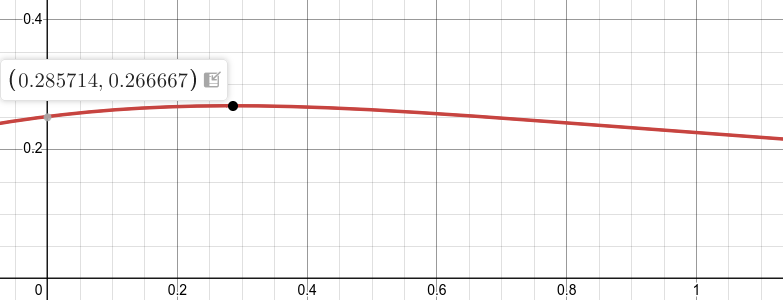
\includegraphics[width=.8\textwidth]{Figures/HW7-8e}
          \caption{SNR versus $d$ Plot}
          \label{fig:1}
        \end{figure}

        As such, the SNR is maximized when $\boxed{d=.285714}$.

    \end{enumerate}

  \item

    \begin{enumerate}

      \item We may begin by expressing the joint PMF as a matrix:

        $$P_{XY}(x,y)=\left[ \begin{matrix} 0 & 1/8 & 3/8 & 1/4\\ 0 & 0 & 1/8 & 0\\ 0 & 0 & 0 & 1/8\\ 0 & 0 & 0 & 0\end{matrix} \right]$$

        Summing the columns, we see that $X=\left\{ 2,3,4 \right\}$ with probabilities $\left\{ \frac{1}{8}, \frac{1}{2}, \frac{3}{8} \right\}$, respectively. Similarly, summing the rows shows us that $Y=\left\{ 1,2,3 \right\}$  with probabilities $\left\{ \frac{3}{4}, \frac{1}{8}, \frac{1}{8} \right\}$, respectively. Using this gives us:

        $$E[X]=\frac{1}{8}(2)+\frac{1}{2}(3)+\frac{3}{8}(4)$$
        $$E[Y]=\frac{3}{4}(1)+\frac{1}{8}(2)+\frac{1}{8}(3)$$

        We solve to get:

        $$\boxed{E[X]=\frac{13}{4}}$$
        $$\boxed{E[Y]=\frac{11}{8}}$$

      \item To find the variances, we begin by writing:

        $$E[X^2]=\frac{1}{8}(2)^2+\frac{1}{2}(3)^2+\frac{3}{8}(4)^2$$
        $$E[Y^2]=\frac{3}{4}(1)^2+\frac{1}{8}(2)^2+\frac{1}{8}(3)^2$$

        This gives us:

        $$E[X^2]=11$$
        $$E[Y^2]=\frac{19}{8}$$

        We then find the variance as:

        $$\text{Var}(X)=E[X^2]-(E[X])^2$$
        $$\text{Var}(Y)=E[Y^2]-(E[Y])^2$$

        This gives us:

        $$\text{Var}(X)=11-\frac{169}{16}$$
        $$\text{Var}(Y)=\frac{19}{8}-\frac{121}{64}$$

        And finally:

        $$\boxed{\text{Var}(X)=.4375}$$
        $$\boxed{\text{Var}(Y)=.4844}$$

      \item We can find the correlation as:

        $$r_{X,Y}=E[XY]=\sum\sum xyP(x,y)$$

        We expand this to get:

        $$r_{X,Y}=\frac{1}{8}(2)(1)+\frac{3}{8}(3)(1)+\frac{1}{4}(4)(1)+\frac{1}{8}(3)(2)+\frac{1}{8}(4)(3)$$

        Solving gives us:

        $$\boxed{r_{X,Y}=\frac{37}{8}=4.625}$$

      \item The covariance may be written as:

        $$\text{Cov}(X,Y)=E[XY]-E[X]E[Y]$$

        Using our obtained values gives us:

        $$\text{Cov}(X,Y)=4.625-\left( 3.25 \right)(1.375)$$
        $$\boxed{\text{Cov}(X,Y)=.1562}$$

      \item We can then write the correlation coefficient as:

        $$\rho_{X,Y}=\frac{\text{Cov}(X,Y)}{\sqrt{\text{Var}(X)\text{Var}(Y)}}$$

        This gives us:

        $$\rho_{X,Y}=\frac{.1562}{\sqrt{(.4375)(.4844)}}$$
        $$\boxed{\rho_{X,Y}=.3394}$$

    \end{enumerate}

\end{enumerate}

\end{document}

